% !TeX program = pdfLaTeX
\documentclass[12pt]{article}
\usepackage{amsmath}
\usepackage{graphicx,psfrag,epsf}
\usepackage{enumerate}
\usepackage{natbib}
\usepackage{textcomp}
\usepackage[hyphens]{url} % not crucial - just used below for the URL
\usepackage{hyperref}
\providecommand{\tightlist}{%
  \setlength{\itemsep}{0pt}\setlength{\parskip}{0pt}}

%\pdfminorversion=4
% NOTE: To produce blinded version, replace "0" with "1" below.
\newcommand{\blind}{0}

% DON'T change margins - should be 1 inch all around.
\addtolength{\oddsidemargin}{-.5in}%
\addtolength{\evensidemargin}{-.5in}%
\addtolength{\textwidth}{1in}%
\addtolength{\textheight}{1.3in}%
\addtolength{\topmargin}{-.8in}%

%% load any required packages here





\begin{document}


\def\spacingset#1{\renewcommand{\baselinestretch}%
{#1}\small\normalsize} \spacingset{1}


%%%%%%%%%%%%%%%%%%%%%%%%%%%%%%%%%%%%%%%%%%%%%%%%%%%%%%%%%%%%%%%%%%%%%%%%%%%%%%

\if0\blind
{
  \title{\bf Bringing Visual Inference to the Classroom}

  \author{
        Adam Loy \\
    Department of Mathematics and Statistics, Carleton College\\
      }
  \maketitle
} \fi

\if1\blind
{
  \bigskip
  \bigskip
  \bigskip
  \begin{center}
    {\LARGE\bf Bringing Visual Inference to the Classroom}
  \end{center}
  \medskip
} \fi

\bigskip
\begin{abstract}
In the classroom, we traditionally visualize inferential concepts
related to inference using static graphics or interactive apps. For
example, there is a long history of using apps to visualize sampling
distributions. Recent developments in statistical graphics have created
an opportunity to bring additional visualizations into the classroom to
hone student understanding. Specifically, the lineup protocol
\citep{Buja-2009bd} provides a framework for students see the difference
between signal and noise. This protocol involves embedding a plot of
observed data in field of null plots. This approach has proved valuable
in visualizing randomization/permutation tests, diagnosing models, and
even conducting valid inference when distributional assumptions break
down. This paper provides an overview of the lineup protocol for visual
inference and how it can be used to hone understanding of key
statistical topics.
\end{abstract}

\noindent%
{\it Keywords:} Statistics education, Statistical graphics, Simulation-based inference, Visualizing uncertainty, Lineup protocol
\vfill

\newpage
\spacingset{1.45} % DON'T change the spacing!

\hypertarget{introduction}{%
\section{Introduction}\label{introduction}}

Could I use the GAISE guidelines to frame the start of this
introduction???

\begin{itemize}
\tightlist
\item
  Recommendation 1: Teach statistical thinking

  \begin{itemize}
  \tightlist
  \item
    simulation-based inference has helped here
  \end{itemize}
\item
  Recommendation 2: Focus on conceptual understanding

  \begin{itemize}
  \tightlist
  \item
    simulation-based inference has helped here
  \item
    applets help students visualize resampling, but not always the big
    picture idea behind inference\ldots{} that's where sesame-street
    logic comes into play\ldots{}
  \end{itemize}
\item
  Recommendation 5: Use technology to explore concepts and analyze data

  \begin{itemize}
  \tightlist
  \item
    apps help
  \item
    lot's of great options (StatKey, Rossman/Chance, Many Shiny
    apps\ldots{})
  \end{itemize}
\end{itemize}

Can we link to hypothetical outcome plots somehow?? Essentially we get
19ish hypothetical outcomes under a model\ldots{}

Recent years have seen a great deal of innovation in how we teach
statistics as we strive to overcome what \citet{Cobb-2007uo} termed
``the tyranny of the computable.'' Most notably, simulation-based
pedagogies for the first course have been proposed and validated
\citep{Cobb-2007uo, Tintle-2011vo, Tintle-2012td, Maurer-2014te, Tintle2014-vt, Hildreth2018}.
These simulation-based pedagogies have also been used in mathematical
statistics \citep{chihara2011, Cobb2011-vz}, and \citet{Tintle2015-yv}
argue that they should be used throughout the entire curriculum.

In addition to changes in how we introduce inference, there have also
been changes in the computational toolkit we use throughout the
statistic curricula. At the introductory level, numerous toolkits are
commonplace depending on the objectives of the course. Web apps are
commonly used in when students may not have access to their own
computers, or to lower the techinical barriers to entry. Examples
include StatKey \citep{Lock2017}, the \emph{Introduction to Statistical
Investigations} applets \citep{tintle2015}, and the shiny apps from
\citet{agresti2017}.

where emphasis is placed on exploring the concepts, but where

Additionally, the GAISE guidelines have led instructors to use
visualization to grapple with higher-dimensional data sets and messier
data\ldots{}

Something about apps\ldots{}

Something about sampling distributions\ldots{}

The goal of this article is to discuss how to incorportate visual
inference into your classroom to help your students differentiate
between different forms of signal and noise, and better understand the
nuances of statistical significance. Section \ref{sec:vizinf} presents
an overview of visual inference, specifically the lineup protocol.
Section \ref{sec:intro} presents examples of how the lineup protocol can
be used in the first course, and Section \ref{sec:othercourses} presents
additional examples throughout the curriculum. We conclude with a brief
summary and discussion in Section \ref{sec:discussion}

\section{Visual inference}
\label{sec:vizinf}

As outlined by \citet{Cobb-2007uo}, most introductory statistics books
teach that classical hypothesis tests consist of (i) formulating null
and alternative hypotheses, (ii) calculating a test statistic from the
observed data, (iii) comparing the test statistic to a reference (null)
distribution, and (iv) deriving a \(p\)-value on which a conclusion is
based. This is still true for the first course after adapting it to
address the new GAISE guidelines regardless of whether a
simulation-based approach is used
\citep[cf.][]{Lock2012, tintle2015, introstats}.

The \emph{lineup protocol} for visual inference has a direct analog for
each of these four steps, as outlined by \citet{Buja-2009bd}. As a first
example of visual inference via the lineup protocol, consider the
creative writing experiment discussed by \citep[pp.~2--14]{ramsey2013}.
The experiment was designed to exploer whether creativity scores were
impacted by the type of motivation (intrinsic or extrinsic). To do this
creative writers were randomly assigned to a questionnaire where they
ranked reasons they write: one questionnaire listed intrinsic
motivations and the other listed extrinsic motivations. After completing
the questionnaire, all subjects wrote a Haiku about laughter which was
graded for creativity by a panel of poets. \citet{ramsey2013} discuss
how to conduct a permutation test for the difference in mean creativity
scores between the two treatment groups. Below, we illustrate the steps
of a visual test.

\begin{enumerate}
\def\labelenumi{\arabic{enumi}.}
\item
  A visual test begins identically to a traditional hypothesis test, by
  clearly stating the competing claims about the model/population
  parameters. In a first course, this could be written as:
  \(H_0: \mu_{\rm intrinsic} - \mu_{\rm extrinsic} = 0\) vs.
  \(H_0: \mu_{\rm intrinsic} - \mu_{\rm extrinsic} \ne 0\).
\item
  The test statistic is a plot displaying an aspect of the data or model
  that allows the observer to differentiate scenarios under the null
  hypothesis from scenarios under alternative hypotheses. Here,
  side-by-side boxplots, or faceted histograms or density plots are
  reasonable choices to display the relevant aspects of the
  distribtions. Figure \ref{fig:data_plot} are boxplots of the original
  creative writing scores by treatment group where a dot is used to
  represent the sample mean for each group.
\end{enumerate}

\begin{figure}
\centering
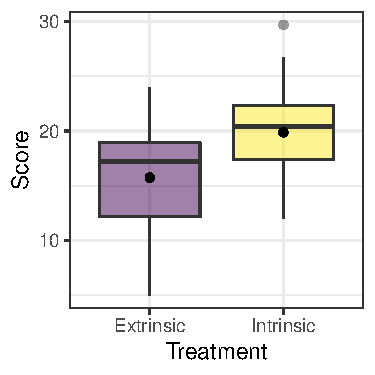
\includegraphics{figs/diff_means_plot.pdf}
\caption{\label{fig:data_plot} Boxplots of the original creative writing
scores by treatment group. The dot represents the mean of each group.}
\end{figure}

\begin{enumerate}
\def\labelenumi{\arabic{enumi}.}
\setcounter{enumi}{2}
\tightlist
\item
  \emph{Null plots} are generated consistently with the null hypothesis
  and the set of all null plots constitutes the reference distribution.
  To facilitate comparison of the data plot to the null plots, the data
  plot should be randomly situtated in the field of null plots. This
  arrangement of plots is called a \emph{lineup}. Figure
  \ref{fig:lineup} shows one possible lineup for the creative writing
  experiment. The 19 null plots were generated via permutation
  resampling, and the data plot was randomly assigned to panel \#4.
\end{enumerate}

\begin{figure}
\centering
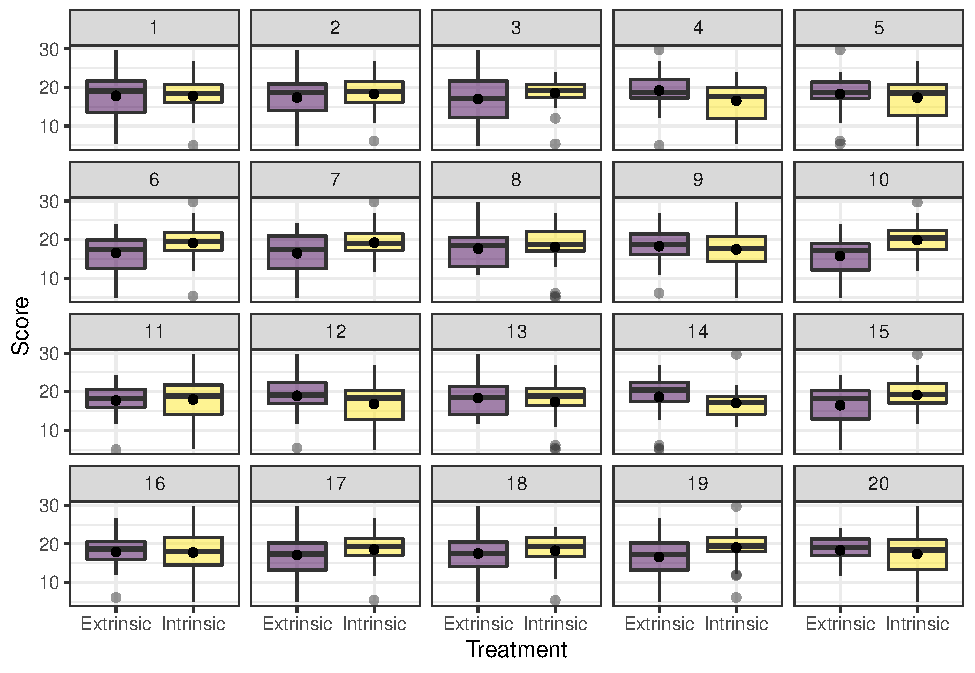
\includegraphics{figs/permute_lineup.pdf}
\caption{\label{fig:lineup} A lineup consisting of 19 null plots
generated via permutation resampling and the original data plot for the
creative writing study. The data plot was randomly placed in panel \#4.}
\end{figure}

\begin{enumerate}
\def\labelenumi{\arabic{enumi}.}
\setcounter{enumi}{3}
\tightlist
\item
  If the null hypothesis is true, then we expect the data plot to be
  indistinguishable from the null plots. Thus, is one is able to
  identify the data plot in panel \#4 of Figure \ref{fig:lineup}, then
  this provides evidence against the null hypothesis. If one wishes to
  calculate a \emph{visual p-value}, then lineups need to be presented
  to a number of independent observers for evaluation. While this is
  possible, we will not discuss this process as the pedagaogical value
  of the lineup protocol is in visualizing signal and noise.
\end{enumerate}

\section{Using visual inference in introductory statistics}
\label{sec:intro}

In this section, we discuss how to incorportate the lineup protocol into
your classroom to clarify common points of confusion. The goal is to
provide examples of how this could be done, not to provide an exhaustive
list of possibilities.

\hypertarget{introducing-simulation-based-inference}{%
\subsection{Introducing (simulation-based)
inference}\label{introducing-simulation-based-inference}}

The strong parallels between visual inference and classical hypothesis
testing make it a natural way to introduce the idea of statistical
significance without getting bogged down in the minutia of \(p\)-values.
In this section, we will outline how we use visual inference to
introduce the concepts behind hypothesis testing without devling into
formal details. To do this, we will continue to discuss the reative
writing experiment introduced in Section \ref{sec:vizinf}.

\hypertarget{interpreting-unfamiliar-plots}{%
\subsection{Interpreting unfamiliar
plots}\label{interpreting-unfamiliar-plots}}

A second way to utilize visual inference in the first course is to help
students build intuition about new and unfamiliar plot types. Two plot
types that we have found introductory students struggle to interpret are
the normal quantile-quantile (Q-Q) plot and the residual plot. In both
situations, the lineup protocol helps students tune their understanding
of what constitutes an ``interesting'' pattern (i.e.~signal).

\hypertarget{q-q-plots}{%
\subsubsection{Q-Q plots}\label{q-q-plots}}

Teaching a novice to interpret a normal Q-Q plot is no easy task,
especially in an algebra-based first course where students can get lost
in the calculation of quantiles rather than focusing on the bigger
picture. Further, Q-Q plots already suffer from a perception problem,
since humans have a tendency to evaluate the shortest (i.e.~orthogonal)
distance, even when asked to evaluate vertical distances
\citep{cleveland1984, robbins2005, sineillusion}. While a detrended
version of the Q-Q plot has been proposed to overcome this difficulty
\citep{Loy2016-fg}, the plot still requires students to calibrate their
intuition. In this paper we will discuss ``classical'' Q-Q plots for
simplicity.

\ldots{}show for smaller sample sizes\ldots{} do i need to cite meeker
and cook??\ldots{}.

\hypertarget{residual-plots}{%
\subsubsection{Residual plots}\label{residual-plots}}

Interpreting residual plots is also fraught with common errors. We have
found that, regardless of our valient attempts to explain what ``random
noise'' or ``random deviations from a model'' might look like, there is
no substitute for first hand experience. In this section we outline a
class activity/discussion that we use to help train students to
interpret residual plots. The full activity can be found in the
supplemental materials.

To begin, we have students fit a simple linear regression model, write
down what a residual is (in both words and using notation), and then
create a first residual plot, such as Figure \ref{fig:residplot}. Next,
we pose the question: ``Does this residual plot provide evidence of a
model deficiency?'' This provides students time to formalize their
decision, especially what features of the residual plot they based their
decision upon.

\begin{figure}

{\centering 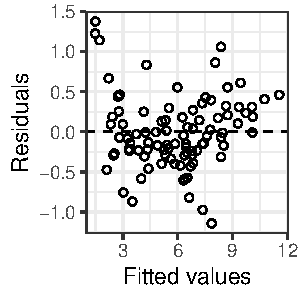
\includegraphics{figs/observed_residual} 

}

\caption{\label{fig:residplot} A residual plot for a simple linear regression model. Is there evidence that the model is insufficient?}\label{fig:residual plot}
\end{figure}

Once students have carefully interpreted the observed residual plot, we
have them generate a lineup where their data plot has been randomly
embedded in a field of null plots, as shown in Figure
\ref{fig:lineupresid}. Here, the null plots have been generated using
the parametric bootstrap, but the residual or non-parametric bootstraps
are other viable choices. We avoid the details of how the null plots
were generated, but this depends on the goals for your class. Once the
lineup has been generated, we ask students to (i) identify which panel
contains the observed residual plot, (ii) describe patterns they
observed in three null plots, and (iii) decide whether/how the observed
residual plot is systematically different from the null plots.

\begin{figure}
\centering
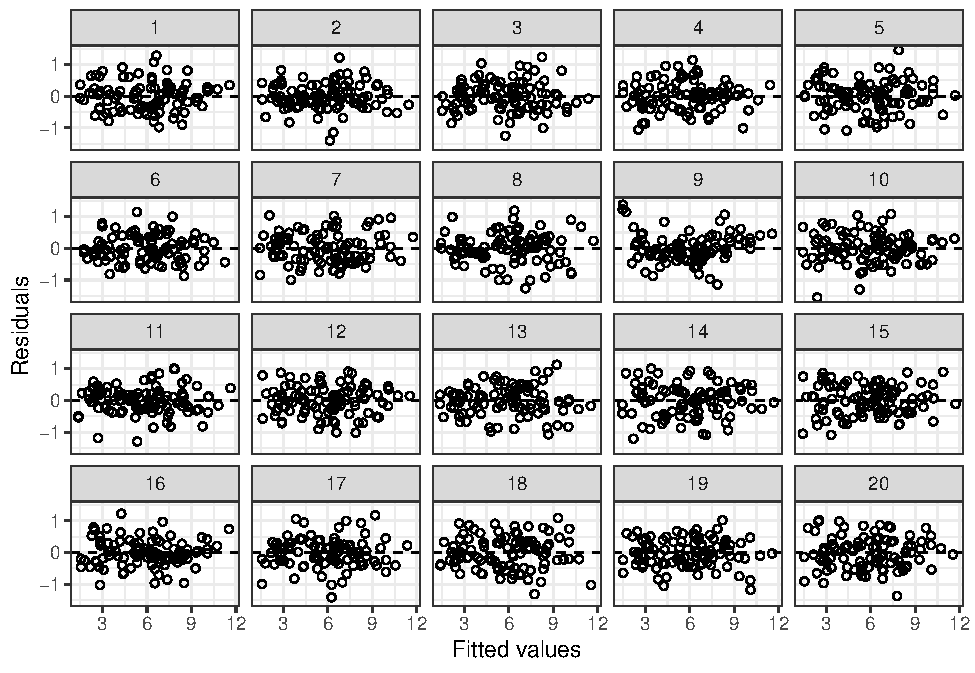
\includegraphics{figs/residual_lineup.pdf}
\caption{\label{fig:lineupresid} A lineup of residual plots. The null
plots are generated via a parametric bootstrap from the fitted model.
The observed data are shown in panel \#9.}
\end{figure}

Teaching tips\ldots{}

\begin{itemize}
\item
  In the above example, the observed residual plot in panel \#9 is
  systematically different from the null plots. While this is one
  example we use in class, we also recommend a parallel example where
  there is no discrepancy between the data and the model.
\item
  Depending on your prefernce and goals, follow-up discussions about the
  design of residual plots could be injected to the end of this
  activity. For example, you could provide students with a second
  version of the lineup where LOESS smoothers have been added to each
  panel and ask students what features of the residual plot this
  highlights.
\item
  An alternative approach would be to have students first use the
  Rorschach protocol to look through a series of null plots, describing
  what they see, and then look at a single residual plot.
\end{itemize}

\section{Using visual inference in other courses}
\label{sec:othercourses}

The utility of visual inference is not restricted to introductory
courses. We have found that whenever a new model is encountered
intuition about diagnostic plots must be rebuilt. As an example we will
consider diagnostics for binary logistic regression models, a common
topic in a second course.

Interpreting residual plots from binary logistic regression is extremely
difficult, as plots of the residuals against the fitted values or
predictors often look similar for adequate and inadequate models. The
lineup protocol provides a framework to have this dicussion. For
example, you can simulate one data set that is appropriate for binary
logistic regression and one that violates the linearity of the logit,
and have your students try to identify the data plot in each situation.

After establishing the pitfalls of ``conventional'' residual plots for
binary logistic regression, you can turn to alternative strategies,
again using the lineup to calibrate student intution with new plot
types. Below we present two examples.

\emph{Binned residuals.} \citet{GelmanHill:2007} recommend using binned
residual plots to explore possible violations of linearity for binary
logistic regression. A binned residual plot is created by calculating
the average residual for a number of bins along the \(x\)-axis. Figure
\ref{fig:binned} shows an example from a simple binary logistic
regression model where the average deviance residual is plotted on the
\(y\)-axis for each of 54 bins on the \(x\)-axis. The bins were set as
with a histogram, and \(\lfloor \sqrt{n} \rfloor\).
\citet{GelmanHill:2007} claim that these plot should behave much like
the familiar standardized residual plots from regression. If this is the
case, then Figure \ref{fig:binned} is indicative of nonlinearity.
However, rather than simply citing \citet{GelmanHill:2007}, a lineup
empowers students to investigate the behavior of this new plot type. A
lineup for these residuals is given in Figure \ref{fig:binnedlineup}. As
suspected, the data plot (panel \#8) clearly stand out from the field of
null plots.

\begin{figure}
\centering
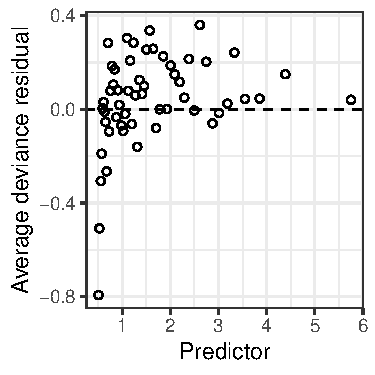
\includegraphics{figs/binned_resid_example.pdf}
\caption{\label{fig:binned} A binned residual plot from a simple binary
logistic regression model. The average deviance residual is plotted on
the \(y\)-axis for each of 54 bins on the \(x\)-axis.}
\end{figure}

\begin{figure}
\centering
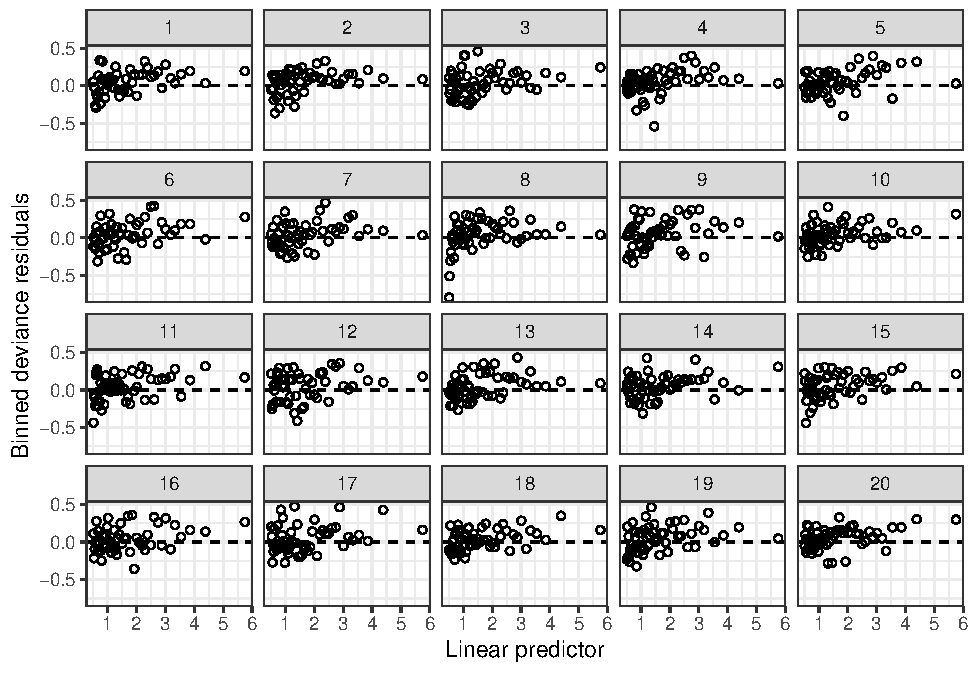
\includegraphics{figs/wells_binned_residuals.pdf}
\caption{\label{fig:binnedlineup} A lineup of binned residual plots from
a simple binary logistic regression model. The observed residuals are
shown in panel \#8 and clearly stand out from the field of null plots,
indicating a problem with linearity.}
\end{figure}

\emph{Empirical logit plots.} A more-common alternative to the binned
residual plot is the empirical logit plot\ldots{}

Need to define briefly\ldots{}

Something about small sample sizes and difficulty interpreting\ldots{}
Let's use one of the Stat2 example here\ldots{} it should be well-known
enough\ldots{}

\begin{figure}
\centering
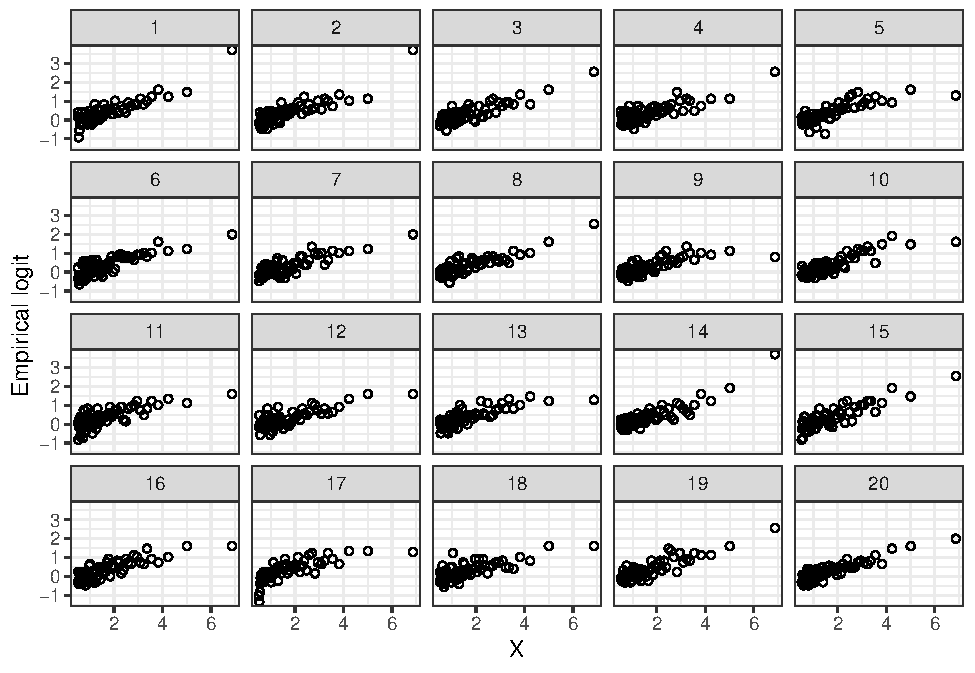
\includegraphics{figs/emp_logit_lineup.pdf}
\caption{\label{fig:emplogitlineup} A lineup of empirical logit plots
from a simple binary logistic regression model. The observed residuals
are shown in panel \#17 and clearly stand out from the field of null
plots, indicating a problem with linearity.}
\end{figure}

In this section we focused on using visual inference to help diagnose
logistic regression models, but the approach is more general. If you
have a plot highlighting some feature(s) of the fitted model, then after
simulating data from a ``correct'' model (i.e.~one without model
deficiencies), you can create a lineup to interrogate the model. For
example, \cite{Loy2017-fo} discuss how visual inference can be used to
diagnose multilevel models.

\hypertarget{discussion}{%
\section{Discussion}\label{discussion}}

\label{sec:discussion}

MENTION PEDAGOGICAL CONSIDERATIONS NOT YET DISCUSSED, HOW TO IMPLEMENT
IN SOFTWARE OR AN APP, IN CLASS V. HOMEWORK, ETC.

A BRIEF GO AND DO PARAGRAPH TO REITERATE THE MESSAGE

\bibliographystyle{agsm}
\bibliography{classroomVizInf.bib}

\end{document}
